\documentclass[presentation]{beamer}
\usepackage[utf8]{inputenc}
\usepackage[T1]{fontenc}
\usepackage{fixltx2e}
\usepackage{graphicx}
\usepackage{longtable}
\usepackage{float}
\usepackage{wrapfig}
\usepackage{rotating}
\usepackage[normalem]{ulem}
\usepackage{amsmath}
\usepackage{textcomp}
\usepackage{marvosym}
\usepackage{wasysym}
\usepackage{amssymb}
\usepackage{hyperref}
\tolerance=1000
\usepackage{graphicx} \DeclareMathOperator{\argmin}{argmin}

\newcommand{\me}{\mathrm{e}}
\providecommand{\e}[1]{\ensuremath{\times 10^{#1}}} 
\providecommand{\mb}[1]{\mathbf{#1}}
\providecommand{\mf}[1]{\mathfrak{#1}}
\providecommand{\ro}[1]{\mathbf{\mathfrak{r}}_o}
\providecommand{\so}[1]{\mathbf{\hat{s}}_o}
\providecommand{\rb}[1]{\mathbf{r}_b}
\providecommand{\rbm}[1]{r_b^{\text{m}}}
\providecommand{\rd}[1]{\mathbf{r}_d}
\providecommand{\mh}[1]{\mathbf{\hat{#1}}}
\providecommand{\bs}[1]{\boldsymbol{#1}} 
\providecommand{\intinf}{\int_{-\infty}^{\infty}}


\newcommand{\under}[2]{\underset{\scriptscriptstyle#1}{#2}}


\usetheme{simple}
\usecolortheme{}
\usefonttheme{serif}
\useinnertheme{}
\useoutertheme{}
\author{Talon Chandler}
\date{March 5, 2018}
\title{Spatio-angular Transfer Functions}

\begin{document}

\maketitle
\begin{frame}[label=sec-1]{$x$-oriented dipole point spread function}
 \begin{center}
   \includegraphics[width=0.8\textwidth]{figs/x.png}
 \end{center}
\end{frame}

\begin{frame}[label=sec-1]{$z$-oriented dipole point spread function}
 \begin{center}
   \includegraphics[width=0.8\textwidth]{figs/z.png}
 \end{center}
\end{frame}

\begin{frame}[label=sec-1]{Point spread functions---Novotny}
 \begin{center}
   \includegraphics[width=0.8\textwidth]{figs/z.png}
 \end{center}
\end{frame}

\begin{frame}[label=sec-1]{Point spread functions---Novotny}
 \begin{center}
   \includegraphics[width=0.8\textwidth]{figs/nov-psf.png}
 \end{center}
\end{frame}

\begin{frame}[label=sec-1]{Only two spherical harmonics in the paraxial spatio-angular point spread function}
 \begin{center}
   \includegraphics[width=0.7\textwidth]{figs/sh.png}
 \end{center}
\end{frame}

\begin{frame}{Paraxial spatio-angular point spread function}
\begin{align*}
      h^*(\rd{}; \mathbf{r}_o, \so{}) \propto ({I_0^*}^2 + 2{I_1^*}^2)Y_0^0(\so{}) + \frac{1}{\sqrt{5}}\left(-{I_0^*}^2 + 4{I_1^*}^2\right)Y_2^{0}(\so{})\label{eq:para}
\end{align*}
\begin{align*}
  {I_0^*} = \left(\frac{\text{NA}}{n_o}\right)^2\left[\frac{2J_1(\tilde{r}_d)}{\tilde{r}_d}\right],
  \hspace{2em}
  {I_1^*} = \left(\frac{\text{NA}}{n_o}\right)^3\left[\frac{2J_2(\tilde{r}_d)}{\tilde{r}_d}\right],
  \end{align*}
  \begin{align*}
  \tilde{r}_d = \frac{2\pi\text{NA}\thinspace r_d}{M\lambda},\hspace{2em}
  \text{NA} = n_o\sin\theta_{\text{max}},\hspace{2em}
  M = \frac{n_o}{n_b}\frac{f_t}{f_o}.
\end{align*}
\end{frame}

\begin{frame}[label=sec-1]{Paraxial spatio-angular PSF and OTF}
 \begin{center}
   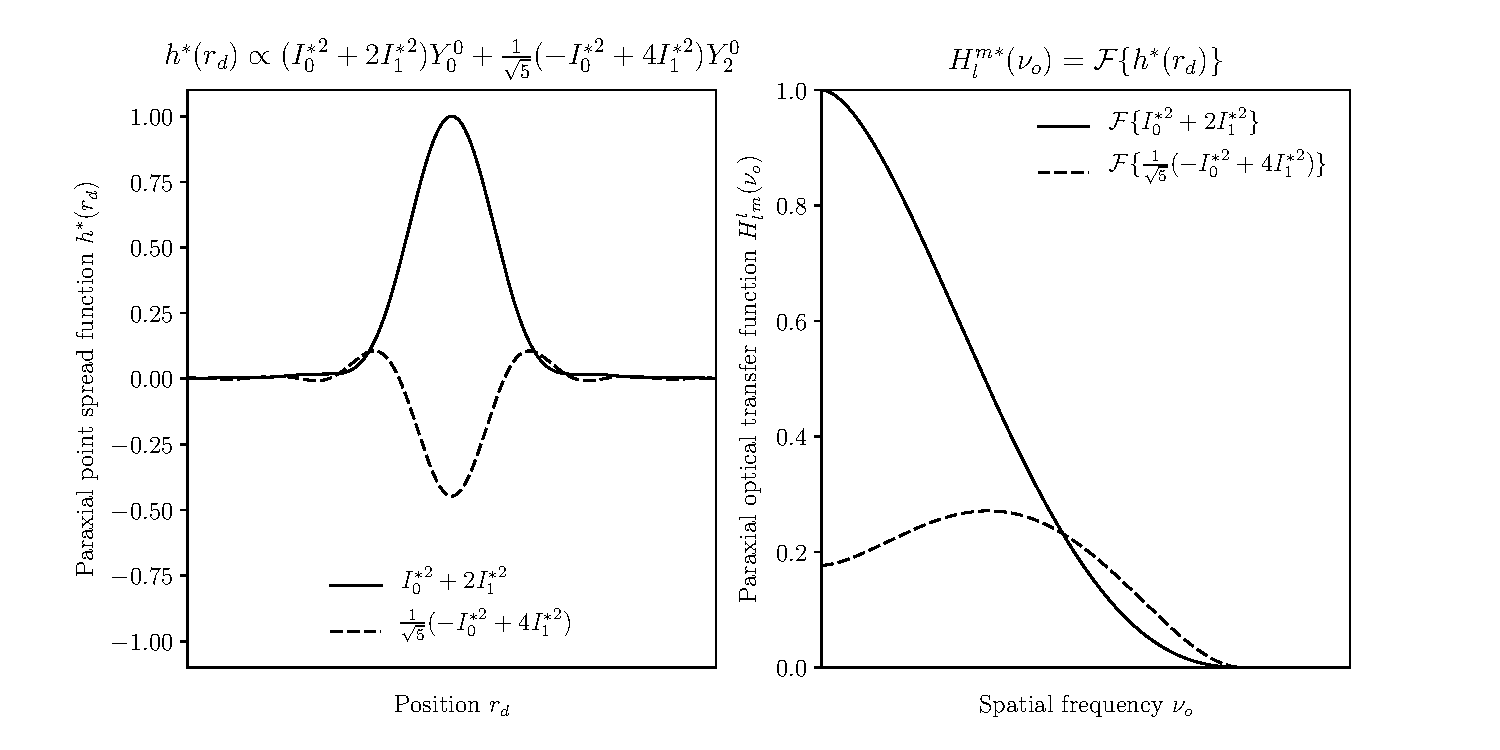
\includegraphics[width=1.0\textwidth]{figs/ft.pdf}
 \end{center}
\end{frame}

\begin{frame}[label=sec-1]{Scalar optics transfer functions---Mertz, Goodman}
 \begin{center}
   \includegraphics[width=.7\textwidth]{figs/mertz.jpg}
 \end{center}
\end{frame}

\begin{frame}[label=sec-1]{Electromagnetic optics transfer functions}
\tikzstyle{block} = [draw, fill=white, rectangle, 
    minimum height=2cm, minimum width=3cm, text width=2cm, align=center]
\tikzstyle{sum} = [draw, fill=white, circle, node distance=4cm]
\tikzstyle{input} = [coordinate]
\tikzstyle{output} = [coordinate]
\tikzstyle{pinstyle} = [pin edge={to-,thin,black}]
\begin{tikzpicture}[auto, node distance=3cm,>=latex]
    \node [input, name=input] {};
    \node [block, align=center] (csf) {CSF\\ $\mb{e}_d(\rd{};\ro{}, \so{})$};
    \node [block,  right of=csf, node distance=6cm] (ctf) {CTF\\ $\mb{e}_b(\rb{};\ro{}, \so{})$};
    \node [block, below of=ctf, node distance=4cm] (otf) {OTF\\ $H_l^m(\bs{\nu})$};
    \node [block, below of=csf, node distance=4cm] (psf) {PSF\\ $h(\ro{}, \so{})$};
    
    \draw [<->] (csf) -- node[name=u, text width=3cm, align=center] {Tube Lens\\ $\mathcal{F}_{\mathbb{R}^2}$} (ctf);        
    \draw [->] (ctf) -- node[name=v, right] {$\mathcal{F}_{\mathbb{S}^2}[\mb{e}_b\star_{\mathbb{R}^2} \mb{e}_b]$} (otf);
    \draw [<->] (psf) -- node[below] {$\mathcal{F}_{\mathbb{R}^3\times\mathbb{S}^2}$} (otf);
    \draw [->] (csf) -- node[name=v, text width=3cm, align=center, left] {Detector\\ $|\mb{e}_d(\rd{};\ro{}, \so{})|^2_{\mathbb{R}^2}$} (psf);
      \end{tikzpicture}
\end{frame}

\end{document}